%TODO: add cliffhanger with preview for next time

%variability
%code-generation
%testing

%modularity? + dependences

%TODO: argumentation/motivation for code generation:
% - misconfiguration caused by transformation/defaults/...

% Make nice A4 pages for print:
%\usepackage{pgfpages}
%\pgfpagesuselayout{resize to}[a4paper,border shrink=5mm,landscape]

\beamertemplatenavigationsymbolsempty

\setbeamertemplate{bibliography item}[text]

\usepackage[type={CC},modifier={by-sa},version={4.0}]{doclicense}

\usepackage[utf8]{inputenc}
\usepackage{hyperref}
\usepackage{breakurl}
\usepackage{graphicx}
\usepackage{pgfplots}
\usepackage{pgf}
\usepackage{tikz}
\usetikzlibrary{positioning}
\usetikzlibrary{arrows}
\usetikzlibrary{decorations.markings}
\usetikzlibrary{calc}
\usetikzlibrary{matrix}
\usetikzlibrary{shapes}
\usetikzlibrary{decorations.pathmorphing}
\usetikzlibrary{fit}
\usetikzlibrary{backgrounds}
\usetikzlibrary{plotmarks}
\usepackage{stmaryrd}
\usepackage{listings}
\usepackage{pdflscape}
\usepackage{perpage}
\usepackage{appendixnumberbeamer}

%\usepackage[thmmarks,amsmath,amsthm]{ntheorem} % already included in beamer
\usepackage{thm-restate}

\usepackage[sort&compress,numbers]{natbib}  % to be have \citet, \citeauthor, \citeyear

\MakePerPage{footnote}

\tikzstyle{o}=[r,ppBlue]
\tikzstyle{r}=[thick,rectangle,align=center]
\tikzstyle{t}=[r,ppTrans] %,font=\bfseries]
\tikzstyle{dd}=[densely dashed]
\tikzstyle{n}=[r,ppBlue]
\tikzstyle{p}=[r,ppRed]
\tikzstyle{ppRed}  =[draw=red,  fill=  red!20]
\tikzstyle{ppBlue} =[draw=blue, fill= blue!20]
\tikzstyle{ppGreen}=[draw=green,fill=green!20]
\tikzstyle{ppTrans}=[draw=none, fill=none]

\usetheme{Warsaw}

\useoutertheme[subsection=true]{smoothbars}
%\useoutertheme[subsection=false]{miniframes}

\definecolor{bblue}{HTML}{D7DF01}	% yellow-ish actually, for better black/white printing
\definecolor{rred}{HTML}{C0504D}
\definecolor{ggreen}{HTML}{9BBB59}
\definecolor{ppurple}{HTML}{9F4C7C}
\definecolor{lightgray}{rgb}{0.3,0.3,0.3}
\definecolor{lightergray}{rgb}{0.9,0.9,0.9}
\definecolor{UniBlue}{RGB}{83,121,170}

\DeclareTextFontCommand\textintro{\normalfont\bfseries\itshape} % nice!
\newcommand{\intro}[2][]
{%
	\textintro{#2}%
}
\newcommand{\empha}[2][]
{%
	\emph{#2}%
}

%\theoremstyle{plain}
\newcounter{reqcounter}
\newtheorem{requirement}[reqcounter]{Requirement}

%setbeamercolor{structure}{fg=violet}

\makeatletter
\def\th@task{%
    \normalfont % body font
    \setbeamercolor{block title example}{bg=orange,fg=white}
    \setbeamercolor{block body example}{bg=orange!20,fg=black}
    \def\inserttheoremblockenv{exampleblock}
  }
\makeatother

\theoremstyle{task}
\newtheorem{task}{Task}

\newenvironment{assignment}%
{%\setbeamercolor{background canvas}{bg=violet}%
%\setbeamercolor{structure}{fg=cyan!90!black}%
 \setbeamercolor{frametitle}{bg=orange,fg=white}
\begin{frame}}%
{\end{frame}}%

\AtBeginSection[]{
  \begin{frame}
  \vfill
  \centering
  \begin{beamercolorbox}[sep=8pt,center,shadow=true,rounded=true]{title}
    \usebeamerfont{title}\insertsectionhead\par%
  \end{beamercolorbox}
  \tableofcontents
  \vfill
  \end{frame}
}




\pgfplotsset{compat=1.14}
\author{Markus Raab}


\date{13.4.2018}

\begin{document}

\renewcommand{\enquote}[1]{\emph{``#1''}} % Cannot be done earlier

%%%%%%%%%%%%%%%%%%%%%%%%%%%%%%%
\begin{frame}
	\titlepage
	\doclicenseThis
\end{frame}

\begin{frame}
	\frametitle{Organization}
	Next dates:
	\begin{description}
		\item[13.4.2018:] \textbf{homework submitted, topics of team exercise}
		\item[27.4.2018:] lecture
		\item[4.5.2018:] lecture
		\item[18.5.2018:] guest lecture
		\item[25.5.2018:] team exercise submitted
		\item[1.6.2018:] lecture
		\item[8.6.2018:] lecture
		\item[15.6.2018:] last corrections of team exercise
		\item[22.6.2018:] test
	\end{description}
\end{frame}


\begin{frame}
	\frametitle{Popular Topics}
	\vspace{-0.5cm}
	\begin{multicols}{2}
	\begin{description}
	\item[4] validation
	\item[4] user interface
	\item[3] tools (benefits?)
	\color{red}
	\item[3] testability
	\color{gray}
	\item[3] complexity reduction (when conf. needed?)
	\item[3] architectural decisions
	\color{black}
	\color{red}
	\item[2] Puppet
	\color{gray}
	\item[2] modularity
	\item[2] environment variables
	\color{black}
	\item[2] documentation
	\color{red}
	\item[2] configuration specification
	\color{gray}
	\item[2] command-line args\color{black}
	\color{red}
	\item[2] code generation
	\color{black}
	\item[1] variability
	\item[1] self-description
	\item[1] round-tripping
	\item[1] early
	\color{gray}
	\item[1] introspection
	\item[1] dependences
	\item[1] auto-detection
	\color{black}
	\item[1] context-awareness
	\item[1] administrators
	\end{description}
	\end{multicols}
\end{frame}

\begin{frame}
	\hspace*{-1cm}\includegraphics[width=\paperwidth]{dot/topics}
\end{frame}

\begin{frame}
	\frametitle{Configuration Access (Recapitulation)}
	\pause

	\ExecuteMetaData[../book/background.tex]{definition-configuration-access}

	\ExecuteMetaData[../book/background.tex]{definition-configuration-access-points}
\end{frame}

\begin{frame}[fragile]
	\frametitle{Trend (Recapitulation)}

	\begin{itemize}[<+-| alert@+>]
	\item alarming trend in number and complexity of configuration settings
	\item sharing, visibility and default value calculation often helps
	\item needs abstraction: configuration specification
	\item but also more courageous decisions and periodical reevaluation
	\item different ways to reduce configuration space
	\end{itemize}
\end{frame}

\begin{frame}
	\frametitle{SpecElektra (Recapitulation)}
	\pause

	\fontsize{18}{0}\selectfont
	\ExecuteMetaData[../book/approach.tex]{definition-spec}
\end{frame}


\begin{frame}
	\frametitle{Modularity (Recapitulation)}
	\pause
	\Large
	\ExecuteMetaData[../book/backend.tex]{definition-modularity}
\end{frame}

\begin{frame}
	\frametitle{Vertical Modularity (Recapitulation)}
	\begin{columns}[c]
	\column{7cm}
	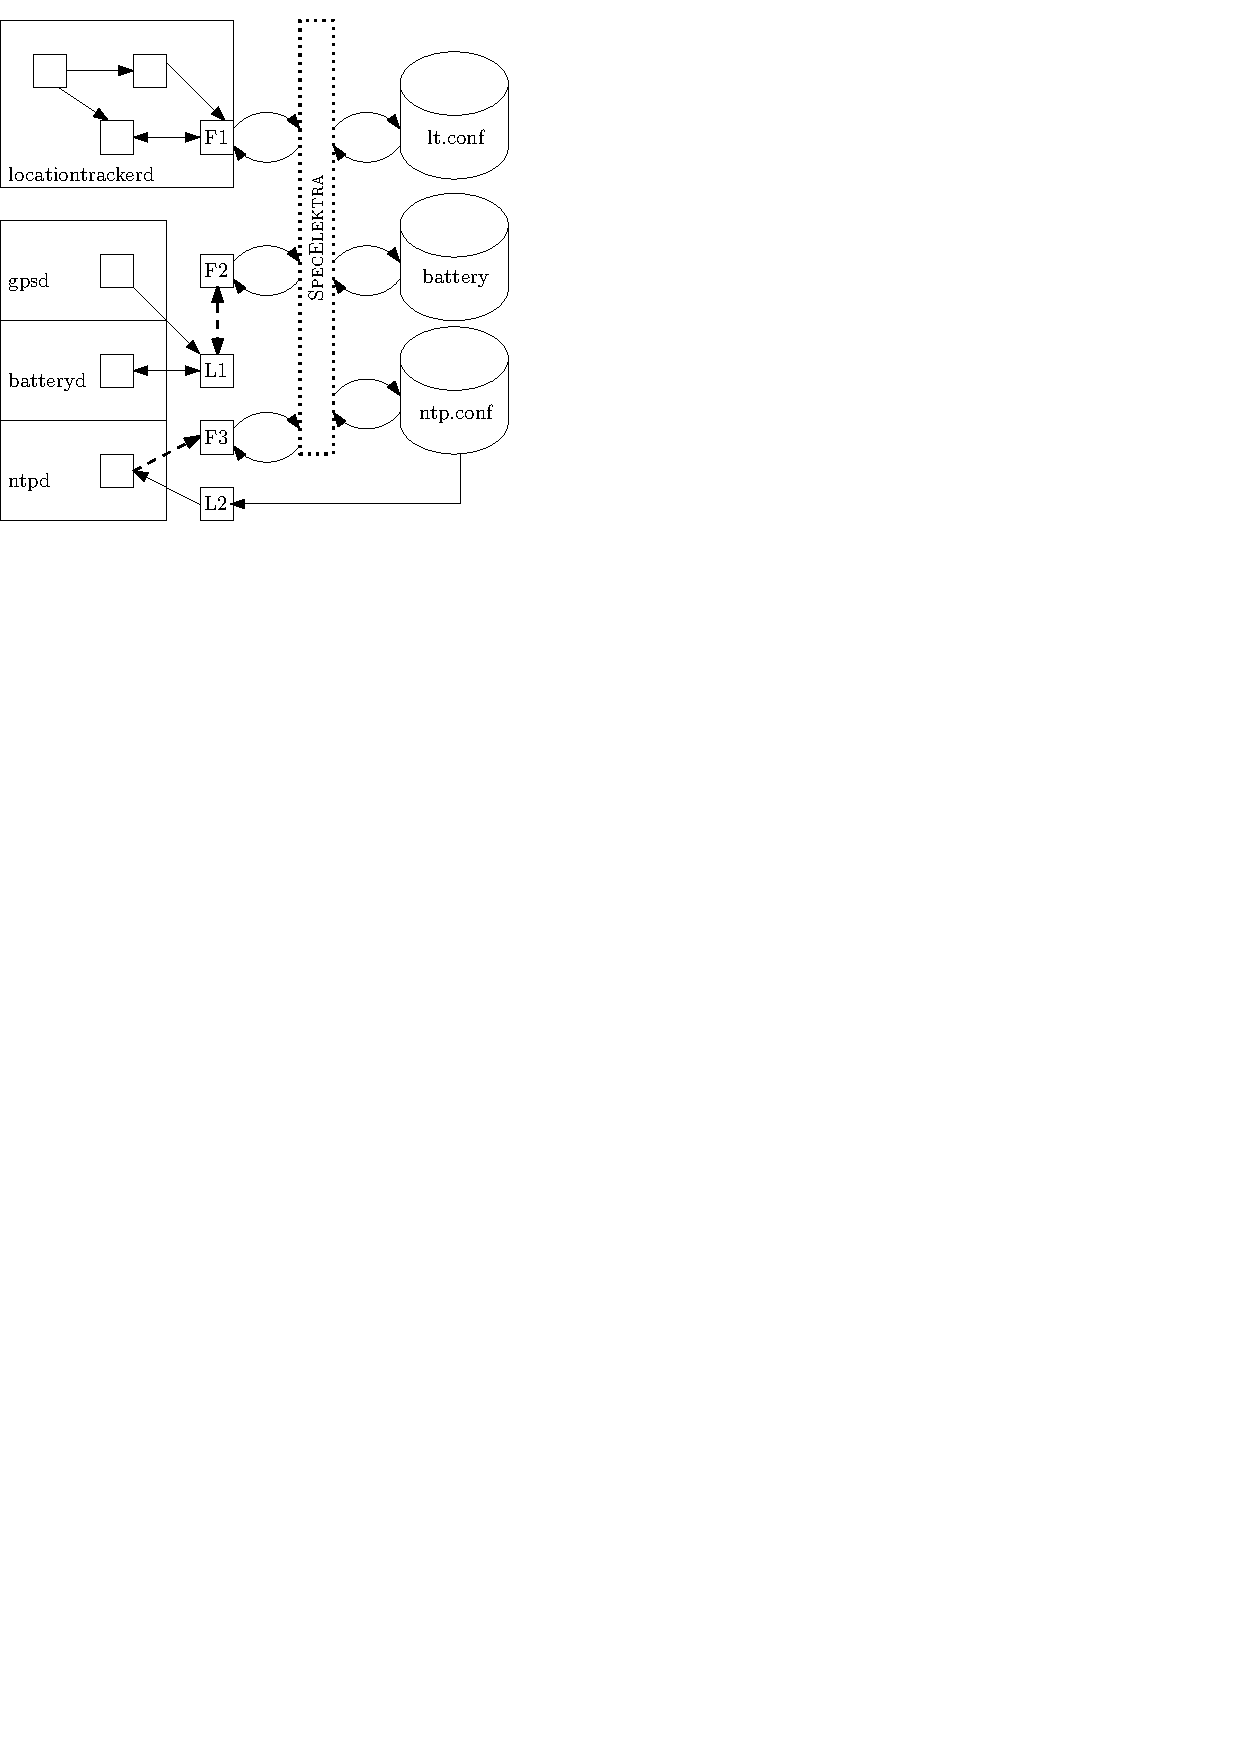
\includegraphics[scale=0.75]{verticalmodularity}
	\column{4cm}
	Needed to keep applications independently.

	Boxes are applications, cylinders are configuration files, F? are frontends or frontend adapters, L? are configuration libraries~\cite{raab2016improving}.
	\end{columns}
\end{frame}


\begin{frame}
	\frametitle{Plugins (Recapitulation)}
	\pause
	\Large
	\ExecuteMetaData[../book/approach.tex]{definition-plugins}
\end{frame}

\begin{frame}
	\frametitle{Introspection (Recapitulation)}
	\pause
	\begin{itemize}
	\item unified get/set access to (meta*)-key/values
	\item access via applications, CLI, GUI, web-UI, ...
	\item access via any programming language (similar to file systems)
	\item GUI, web-UI can semantically interpret metadata
	\end{itemize}
\end{frame}


%%%%%%%%%%%%%%%%%%%%%%%%%%%%%%%%%%%%%%%%%% 
\section{Code Generation}

\subsection{Why?}

\begin{assignment}
	\begin{task}
	How to ensure that configuration access points match with present configuration settings?
	\end{task}
\end{assignment}

\begin{frame}
	\frametitle{Rationale (Partly Recapitulation)}
	Configuration Specification:
	\begin{itemize}
	\item without specification you and others do not even know which settings are available
	\item needed for any further techniques we will discuss:
		\begin{itemize}
		\color{red}
		\item code generation guarantees that configuration access points match with specification
		\item validation guarantees that configuration settings match with specification
		\end{itemize}
	\item essential for \intro[no-futz computing]{no-futz computing}~\citet{holland2001nofutz}
	\item the foundation for any advanced tooling like configuration management tools
	\item needed as communication of producers and consumers of configuration
	\end{itemize}
\end{frame}

\begin{assignment}
	\begin{task}
	Brainstorming: Which artefacts can we produce with code generation?
	\end{task}
\end{assignment}

\begin{frame}
	Artefacts:
	\begin{itemize}
	\item generate examples/documentation
	\item auto-completion/syntax highlighting/IDE support
	\item tooling (GUI, Web UI)
	\item validation code
	\item configuration management tool code
	\item configuration access APIs
	\end{itemize}
\end{frame}

\begin{frame}[fragile]
	\frametitle{Current Challenges}
	Configuration Access Code usually has:
	\begin{itemize}
	\item code duplications
	\item hard-coded default values
	\item unexpected transformations
	\item no introspection facilities
	\end{itemize}
	\begin{example}
	\begin{code}[gobble=4,language=C++]
	if (!strcasecmp(token, "on")) {
		*var = 1;
	} else {
		*var = 0;
	} /* src/cache_cf.cc from Squid */
	\end{code}\end{example}
\end{frame}

\begin{frame}
	\frametitle{Goal}

	\begin{goal}
	Configuration settings should adhere the specification from source to destination.
	\end{goal}

	\begin{restatable}{requirement}{reqGeneration}
	The specification must enable code generation and inconsistencies must be ruled out during compilation.
	\end{restatable}
\end{frame}


\subsection{How?}

\begin{frame}
	\frametitle{Code Generation}

	\ExecuteMetaData[../book/approach.tex]{code-generation}
\end{frame}

\begin{frame}
	\frametitle{Possible Properties}
	For example, SpecElektra has following properties:
	\begin{description}
	\item[type] represents the type to be used in the emitted source code.
	\item[opt] is used for short command-line options to be copied to the namespace \namespace{proc}.
	\item[opt/long] is used for long command-line options, which differ from short command-line options by supporting strings and not only characters.
	\item[readonly] yields compilation errors when developers assign a value to a contextual value within the program.
	\item[default] enables us to start the application even if the backend does not work.
	\end{description}
\end{frame}

\begin{frame}[fragile]
	With the specification:
	\par
	\begin{code}[gobble=4]
	[foo/bar]
	  default:=Hello
	  type:=string
	  opt:=b
	  readonly:=1
	\end{code}
	\par
	\elektra{Gen} gives the user read-only access to the object ^env.foo.bar^:
	\par
	\begin{code}[language=Cpp]
	std::cout << env.foo.bar;
	env.foo.bar = "Other world"; // comp. error
	\end{code}
	\par
	\small
	Line~1 prints the configuration value of ^/foo/bar^ or ^"Hello"^ (without quotes) by default.
	When invoking the application with ^application -b "This world"^, the application would print ^"This world"^ (without quotes).
	Line~2 leads to a compilation error because of the property \property{readonly}.
\end{frame}

\begin{frame}
	\frametitle{KeySet (Recapitulation)}

	The common data structure between plugins:
	\vspace{1cm}

	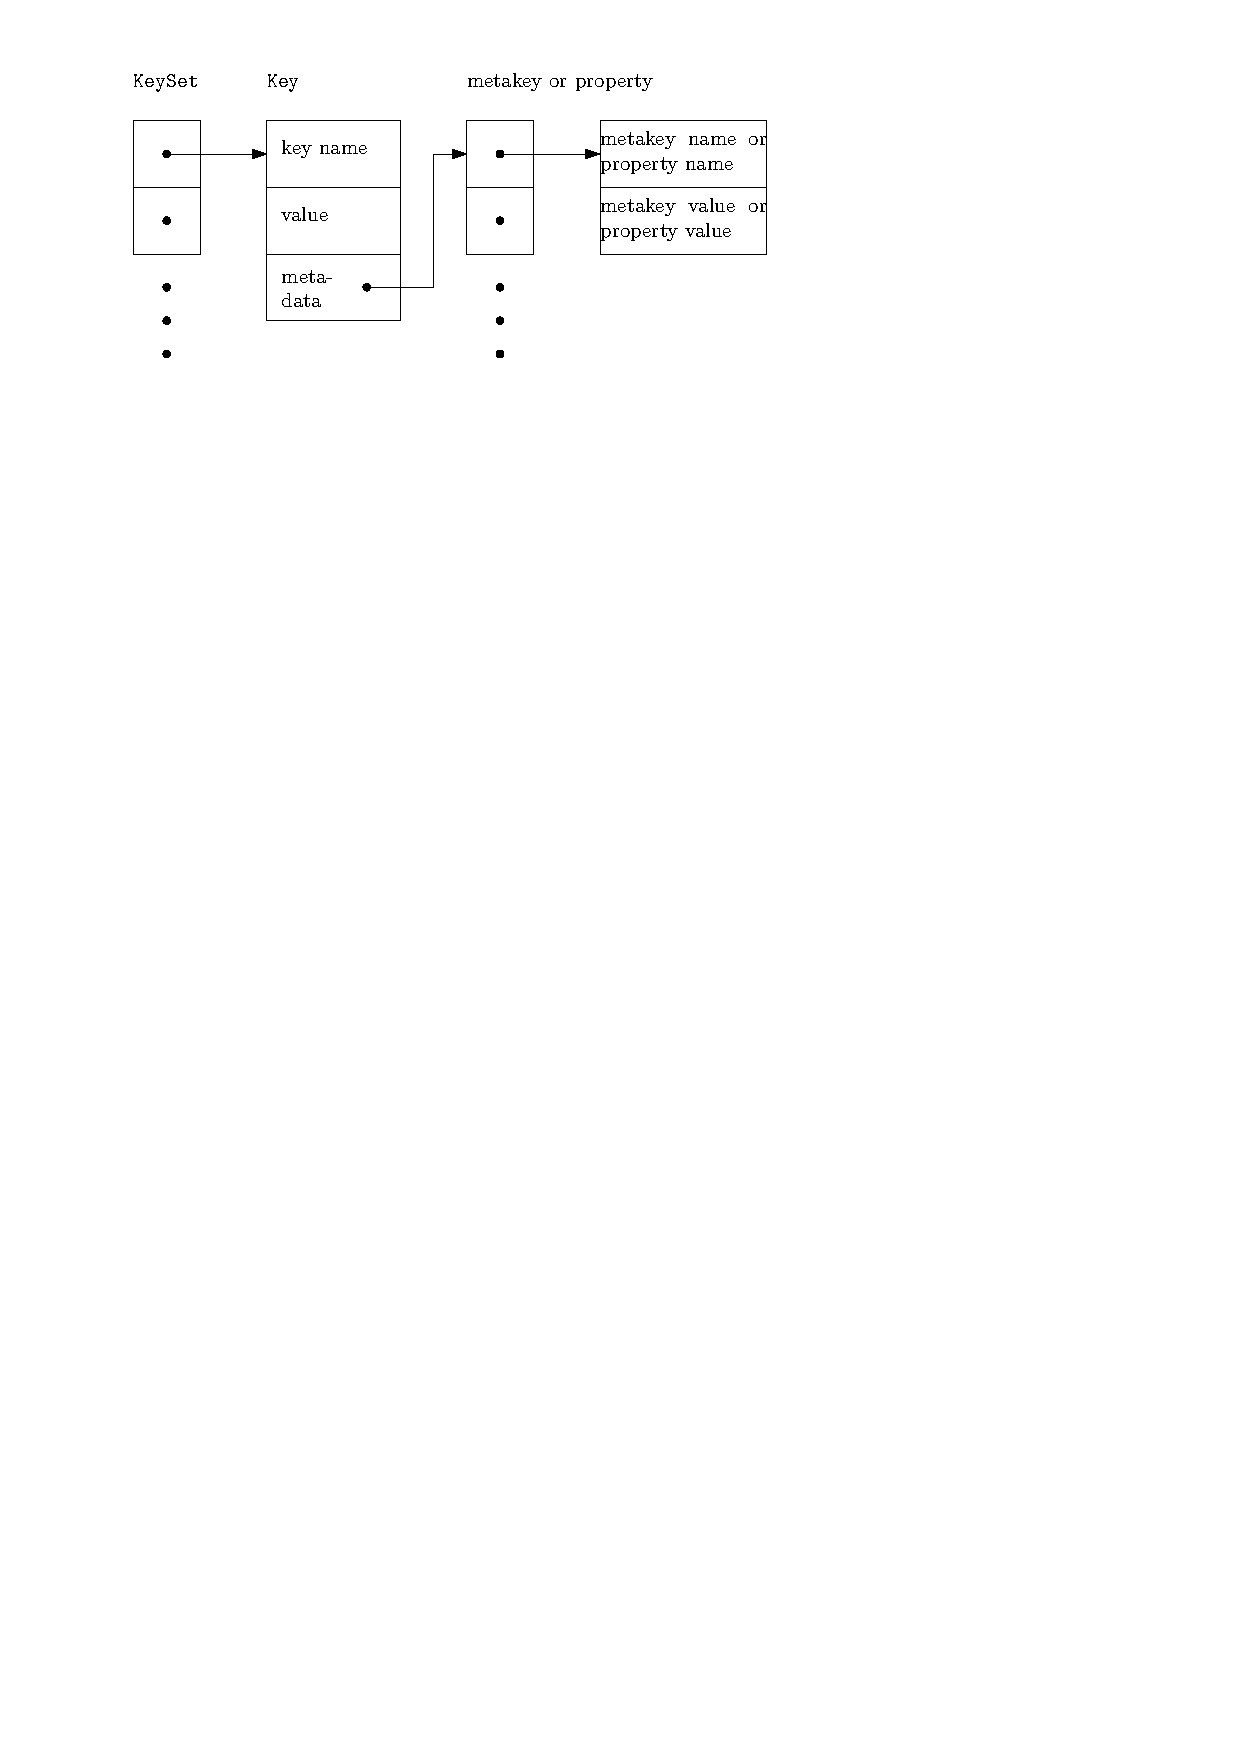
\includegraphics{keyset}
\end{frame}

\begin{frame}[fragile]
	\frametitle{KeySet Generation}
	\begin{alertblock}{Question}
	Idea: What if the configuration file format grammar describes source code?
	\end{alertblock}
	\pause

	\begin{grammar}
	<KeySet> ::= \lq ksNew'\WhiteSpace(' \{ <Key> \lq , \LineBreak'  \}  \{ \lq\WhiteSpace' \} \lq KS\_END);'

	<Key> ::= \lq keyNew \WhiteSpace ('' ' <key name> \lq ''  , \LineBreak' [ <Value> ] <properties> \lq KEY_END)'

	<Value> ::=  \{ \lq\WhiteSpace' \} \lq KEY\_VALUE, \WhiteSpace '' ' <configuration value> \lq ''  , \LineBreak'

	<properties> ::= \{ \{ \lq\WhiteSpace' \} <property> \lq , \LineBreak' \}

	<property> ::=  \lq KEY\_META, \WhiteSpace " ' <property name> \lq "  , \WhiteSpace " ' <property value> \lq " '
	\end{grammar}
\end{frame}

\begin{frame}[fragile]
	\frametitle{Example}
	Given the key ^spec:/slapd/threads/listener^, with the configuration value ^4^ and the property $\property{default} \mapsto 1$, \elektra{Gen} emits:

	\begin{code}[gobble=4,language=Cpp]
	ksNew (keyNew ("spec:/slapd/threads/listener",
		       KEY_VALUE, "4",
		       KEY_META, "default", "1",
		       KEY_END),
	       KS_END);
	\end{code}

	\pause
	\begin{alertblock}{Finding}
	We have source code representing the settings.
	And if we instantiate it, we have a data structure representing the settings.
	Plugins emitting such ``configuration files'' are code generators.
	\end{alertblock}
\end{frame}

\begin{frame}[fragile]
	\frametitle{Implementation Strategies}

	\begin{itemize}
	\item Using ^print^ (only for very small generators)
	\item Using generative grammars
	\begin{code}[gobble=4,language=Cpp]
	query = '{' >> *(pair) > '}';
	pair = '{' >> key_name > '=' >> key_value >>
	       *('{' >> metakey_name > '=' >> metakey_value > '}')
	       > '}';
	\end{code}
	\item Using template languages (RubyERB, Cheetah, GNU AutoGen)
	\begin{code}[gobble=4,language=Python,basicstyle=\ttfamily\tiny,numberstyle=\ttfamily\tiny\color{blue}]
	@for n in hierarchy.name.split('/')[1:-1]
	namespace $support.nsnpretty($n)
	{
	class ${hierarchy.prettyclassname(support)}
	{
	typedef $support.typeof($hierarchy.info) type;
	@if $support.typeof($hierarchy.info) != "kdb::none_t"
	static type get(kdb::KeySet &ks, kdb::Key const& spec)
	{
		type value $support.valof($hierarchy.info)
		Key found(ckdb::ksLookup(ks.getKeySet(), *spec,
					ckdb::elektraLookupOptions::KDB_O_SPEC));
		return found.get<$support.typeof($hierarchy.info)>();
	}
	\end{code}
	\end{itemize}
\end{frame}

\begin{frame}[fragile]
	\frametitle{Which Configuration Access API?}

	First approach, one class (or function) per configuration setting:
	\\[1em]
	\begin{code}[gobble=4,language=Cpp]
	class SlapdThreadsListener : public Value<long,
		WritePolicyIs<ReadOnlyPolicy>> {
		... keyNew ("/slapd/threads/listener",
			    KEY_META, "type", "long",
			    KEY_META, "readonly", "1",
			    KEY_END) ...
	};
	\end{code}
\end{frame}

\begin{frame}[fragile]
	\frametitle{Which Configuration Access API?}

	Bad idea, manual instantiation and long names necessary:
	\\[1em]
	\begin{code}[gobble=4,language=Cpp]
	KeySet config;
	Context c;
	long foo ()
	{
		SlapdThreadsListener slapdThreadsListener (config, c);
		slapdThreadsListener++;
		return slapdThreadsListener;
	}
	\end{code}
\end{frame}

\begin{frame}[fragile]
	\frametitle{Which Configuration Access API?}

	Use hierarchy with namespaces or nasted classes:
	\\[1em]
	\begin{code}[gobble=4,language=Cpp]
	namespace slapd
	{
	namespace threads
	{
	class Listener : public Value<long> {};
	}  // <continues on the next page>
	class Threads : public Value<none_t>
	{threads::Listener listener;};
	}  // end namespace slapd
	class Slapd : public Value<none_t>
	{slapd::Threads threads;};
	class Environment {Slapd slapd;};
	\end{code}
\end{frame}

\begin{frame}[fragile]
	\frametitle{Which Configuration Access API?}

	Much easier to use:
	\begin{code}[gobble=4,language=Cpp]
	long foo(slapd::Threads const & threads)
	{
		threads.listener++;
		Context & c = threads.context (); // access context
		return threads.listener;
	}

	int main()
	{
		KeySet config;
		Context c;
		Environment env (config, c);
		long x = foo (env.slapd.threads);
	}
	\end{code}
\end{frame}

\begin{frame}[fragile]
	\frametitle{Which Configuration Access API?}

	In C, we use identifiers to be passed to the API:
	\\[2em]
	\begin{code}[gobble=4,language=Cpp]
	elektraGetString (elektra, ELEKTRA_TAG_X);
	\end{code}
	Where ^ELEKTRA_TAG_X^ is a struct for that type.
\end{frame}

\begin{frame}
	Guarantees by code generation:
	\begin{itemize}
	\item Every configuration setting is specified.
	\item Configuration access with defaults is always successful.
	Reason: We compile in a KeySet and use it if everything else fails.
	\end{itemize}
	\vspace{3em}
	Missing Guarantee: Is every specified setting actually used?
\end{frame}



%%%%%%%%%%%%%%%%%%%%%%%%%%%%%%%%%%%%%%%%%% 
\section{Introspection vs. Generation}

\subsection{}

\begin{frame}
	\begin{alertblock}{Question}
	Introspection vs. Code Generation?
	\end{alertblock}
\end{frame}

\begin{frame}
	Limitations of introspection:
	\begin{itemize}
	\item no static checks
	\item no whole-program optimizations (API barriers)
	\end{itemize}
\end{frame}

\begin{frame}
	Overhead without code generation (=backend) is $1.8$x higher~\cite{raab2015kps}:
	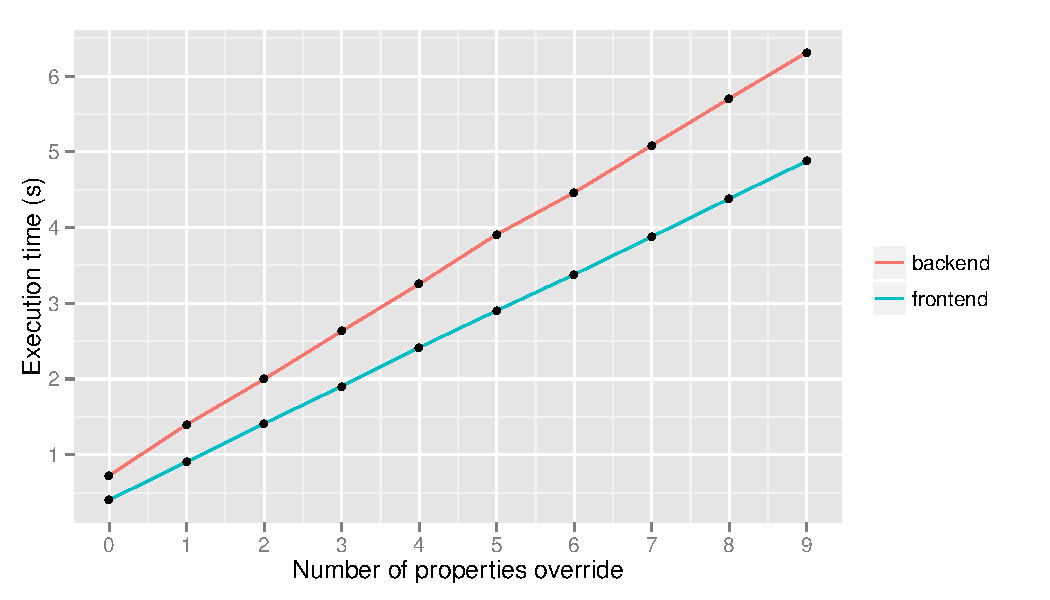
\includegraphics[width=\textwidth]{mean2}
\end{frame}

\begin{frame}
	But it might not matter because configuration access might not be a bottleneck~\cite{raab2015kps},
	for example, a word counting application:

	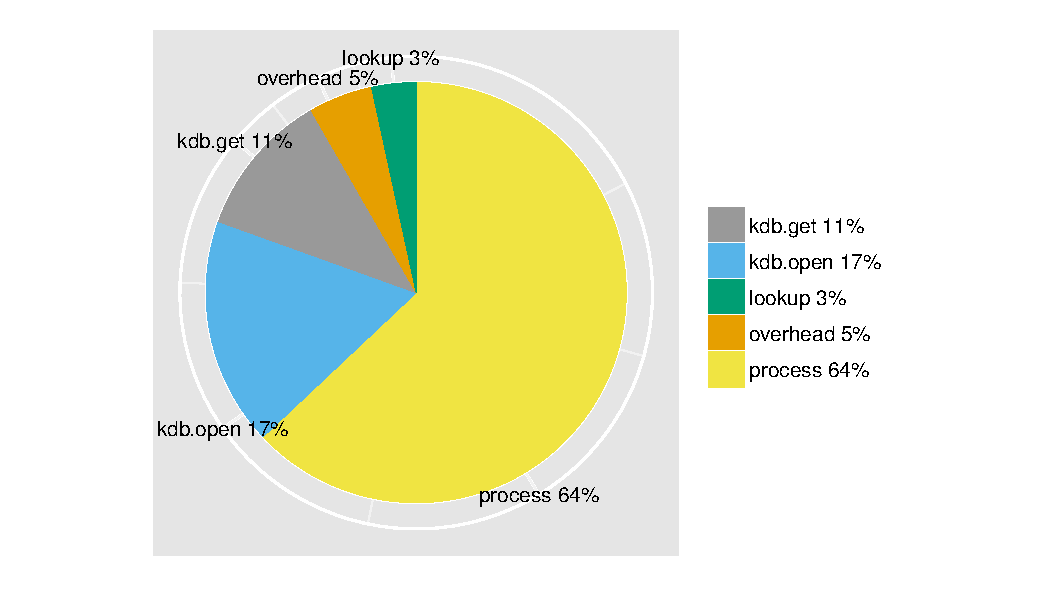
\includegraphics[width=\textwidth]{wc}

	But: \pause
	Configuration access points within loops might be a bottleneck.
\end{frame}

\begin{frame}
	Advantages of introspection:
	\begin{itemize}
	\item specification can be updated live on the system without recompilation
	\item tooling has generic access to all specifications
 	\item new features the key database (e.g., better validation) are immediately available consistently
	\end{itemize}
	\vspace{1em}
	\begin{alertblock}{Implication}
	We generally prefer introspection
	\end{alertblock}
	\vspace{1em}
	\begin{restatable}{requirement}{reqIntrospection}
	Configuration settings and specifications must be introspectable.%
	\end{restatable}
\end{frame}


%%%%%%%%%%%%%%%%%%%%%%%%%%%%%%%%%%%%%%%%%% 
\section{Testability}

\subsection{}

\begin{frame}
	\begin{alertblock}{Question}
	What do we want to test?
	\end{alertblock}

	\pause
	\begin{itemize}
	\item Settings do what they should
	\item Settings are properly validated
	\item Functionality with different settings
	\item Regression tests~\cite{qu2008configuration}
	\pause
	\item Are all settings implemented?
	\item Are all settings used in tests?
	\item Are there unused settings in the code?
	\end{itemize}
\end{frame}

\lstDeleteShortInline^
\begin{frame}
	\frametitle{\cite{jin2014configurations}}

	\begin{itemize}
	\item Wants to improve configuration-ware testing and debugging
	\item Manual investigations for three applications
	\item Finds 1957 settings in Firefox ($2^{846} * 3^{1111}$) and \\
		36322 in LibreOffice ($2^{4433} * 3^{31889}$)
	\item Finds unused settings: settings only in the source code
	\item Finds unsynchronized configuration settings (see in ``early'')
	\end{itemize}

	\begin{requirement}
	Configuration setting traceability is a necessity.
	\end{requirement}

	\begin{alertblock}{Idea}
	Code generation helps to trace settings and to find unused settings.
	\end{alertblock}
\end{frame}
\lstMakeShortInline[postbreak=,keywordstyle={},showspaces=no]^
%XXX

%Other requirements they have:
%\begin{frame}
%	\frametitle{Requirements \cite{jin2014configurations}}
%	\begin{requirement}
%	Configuration Modeling Should Merge Multiple Layers.
%	\end{requirement}
%	\begin{requirement}
%	Analysis Tools Need to Cross the Programming Language Barrier
%	\end{requirement}
%	\begin{requirement}
%	Configuration State Capture or Approximation Techniques are Needed
%	\end{requirement}
%\end{frame}


\begin{frame}
	\frametitle{Find Unused Settings}

	%contextual value not yet introduced:
	%\ExecuteMetaData[../book/implications.tex]{algorithm-first}
	The first (optional) step of the algorithm is:
	\begin{itemize}
	\item Run all tests with code coverage.
	\item Check if generated code is executed.
	\item If it is, we know that the configuration setting is used in a test case.
	Otherwise, we know it is not tested by the test suite.
	All these untested configuration settings are remembered as candidates for the second step.
	\end{itemize}
\end{frame}

\begin{frame}[fragile]
	\small
	\fontsize{10}{0}\selectfont
	\begin{code}[gobble=4,language=Cpp]
	KeySet findUnusedSettings (KeySet untestedSettings,
				   KDB kdb,
				   Builder build)
	{
	   KeySet unusedSettings = {};
	   KeySet configurationSpecification;
	   kdb.get (configurationSpecification);

	   for (candidate: untestedSettings)
	   {
	       configurationSpecification.remove (candidate);
	       kdb.set (configurationSpecification);
	       build.recompile ();
	       if (build.wasSuccessful ())
	       {
	          unusedSettings.append (candidate);
	       }
	       configurationSpecification.append (candidate);
	   }

	   kdb.set (configurationSpecification);
	   return unusedSettings;
	}
	\end{code}
\end{frame}

\begin{frame}[fragile]
	\frametitle{Conclusion}
	\begin{itemize}
	\item Challenges: duplications, transformations, ...
	\item Configuration access APIs with code generation
	\item Guarantees of configuration access points
	\item We reuse properties of SpecElektra (^type^, ^default^)
	\item We prefer hierarchies and tags to long function names
	\item Usually introspection preferred, except for static type safety
	\end{itemize}
\end{frame}

\begin{frame}
	\frametitle{Preview}
	\begin{itemize}
	\item Puppet-Libelektra talk
	\item Early Detection of Misconfiguration
	\end{itemize}
\end{frame}



%%%%%%%%%%%%%%%%%%%%%%%%%%%%%%%%%%%%%%%%%% 
\nocite{raab2017introducing}

\appendix

\begin{frame}[allowframebreaks]
	\bibliographystyle{plainnat}
	\bibliography{../shared/elektra.bib}
\end{frame}

\end{document}


